% Template mimicking the Linnaeus University powerpoint template
% https://lnu.se/en/medarbetare/support-and-service/communications-and-marketing/Designmanual/templates/

\documentclass[english,9pt]{Linnaeus}
\usepackage{babel}
\usepackage{braket}
\usepackage{array,booktabs,times,mathptmx}
\usepackage{tikz}
\usepackage{amsfonts} % Para \mathbb
\usepackage{quantikz}

\usepackage{tikz-3dplot}
\usetikzlibrary{shapes,arrows.meta,calc}


\usetikzlibrary{shapes.symbols}
\usetikzlibrary{calc,arrows.meta}

\newcommand{\drawparal}[7]{ % pos_x, pos_y, v_x, v_y, v_z, label, id
  \begin{scope}[shift={(#1,#2)}]
    \coordinate (O) at (0,0);
    \coordinate (A) at #3; % x-vector
    \coordinate (B) at #4; % y-vector
    \coordinate (C) at #5; % z-vector
    \coordinate (Vab) at ($ (A) + (B) $);
    \coordinate (Vac) at ($ (A) + (C) $);
    \coordinate (Vbc) at ($ (B) + (C) $);
    \coordinate (Vabc) at ($ (A) + (B) + (C) $);
    % Outer contours
    \draw[line width=0.8pt, contour] (A) -- (Vab) -- (B);
    \draw[line width=0.8pt, contour] (B) -- (Vbc) -- (C);
    \draw[line width=0.8pt, contour] (C) -- (Vac) -- (A);
    \draw[line width=0.8pt, contour] (Vab) -- (Vabc);
    \draw[line width=0.8pt, contour] (Vbc) -- (Vabc);
    \draw[line width=0.8pt, contour] (Vac) -- (Vabc);
    % Inner axes with arrows
    \draw[eje] (O) -- (A);
    \draw[eje] (O) -- (B);
    \draw[eje] (O) -- (C);
    % Label positioned in the middle of the front-facing face
    \node[anchor=center, inner sep=1.5pt] at ($ 0.5*#3 + 0.5*#4 $) {#6};

    % Define target coordinate for connection lines (origin of each para, global scope)
    \global\coordinate (#7_orig) at (0,0);
  \end{scope}
  }

  % Uncomment below for specific features

  % If you want to use bibtex uncomment the lines below
  %\usepackage{natbib}
  %    \bibpunct{(}{)}{;}{a}{}{,}
  %    \renewcommand{\bibfont}{\footnotesize}        
  %    \newcommand{\newblock}{.}

  % If you figures are in another folder
  %\graphicspath{{./Figures/}}

  % To reset the font in all tables
  %\let\oldtabular\tabular 
  %\renewcommand{\tabular}{\tiny\oldtabular} 

  \author[S1e7J]{\textbf{Sergio Montoya Ramírez}}
  \institute{s.montoyar2@uniandes.edu.co}
  \title{\LARGE \textbf{RCWA4D: Explicación del Metodo y como Utilizarlo}}
  \date{}


  \begin{document}

  \begin{frame}[plain]
    \titlepage
  \end{frame}

  \setbeamercolor{background canvas}{bg=white}

  \begin{frame}
    \frametitle{RCWA es un método semi-analítico; en particular, parte estructuras complejas en escalones uniformes}
    \begin{columns}
      \begin{column}{0.5\textwidth}
        En vez de tomar el artefacto como conjunto, RCWA parte en capas uniformes en la dirección $z$. Además, cada uno de estos escalones debe ser:
        \begin{itemize}
          \item Periódico en el plano $x-y$
          \item Homogéneo en dirección $z$
        \end{itemize}
        \cite{empossible_rcwa}
      \end{column}
      \begin{column}{0.5\textwidth}
        \begin{figure}
          \begin{center}
            \includegraphics[width=0.95\textwidth]{./imgs/simplification.png}
          \end{center}
        \end{figure}
      \end{column}
    \end{columns}
  \end{frame}

  \begin{frame}[allowframebreaks]
    \frametitle{RCWA trabaja en el espacio reciproco y se recolecta en vectores}

    \begin{align*}
      E_i (x, y, z) &= \sum_{g \in \mathcal{G}} E_i(g; z)e^{i(k_x(g)x + k_y(g)y)}\\
      H_i (x, y, z) &= \sum_{g \in \mathcal{G}} H_i(g; z)e^{i(k_x(g)x + k_y(g)y)}\\
      e_i = \begin{bmatrix}E_i(g^{(1)})\\ E_i(g^{(2)})\\ \vdots\\ E_i(g^{(i)})\end{bmatrix};&\ 
        h_i = \begin{bmatrix}H_i(g^{(1)})\\ H_i(g^{(2)})\\ \vdots\\ H_i(g^{(i)})\end{bmatrix}
    \end{align*}

    Con $g$ un subconjunto de vectores base de la red reciproca para resolver la ecuacion.
  \end{frame}

  \begin{frame}
    \frametitle{Dado que trabajamos en vectores esto se convierte en un problema de algebra lineal}
    \begin{align*}
      \mathbf{s}(\hat{z}) = \begin{bmatrix}e_x(\hat{z})\\ e_y(\hat{z})\end{bmatrix} &= W e^{-\Lambda \hat{z}}c^+ + We^{\Lambda \hat{z}} c^-\\
        \mathbf{u}(\hat{z}) = \begin{bmatrix}h_x(\hat{z})\\ h_y(\hat{z})\end{bmatrix} &= - V e^{-\Lambda \hat{z}}c^+ + Ve^{\Lambda \hat{z}} c^-
    \end{align*}
    Donde los elementos son\cite{lou_fan_2025}

    \begin{itemize}
      \item \textbf{$W, V$}: Matrices de eigenvectores.
      \item \textbf{$\Lambda$}: Matriz de constantes de propagación.
      \item \textbf{$e^{\pm \Lambda \hat{z}}$}: Términos de fase y atenuación/ganancia.
      \item \textbf{$c^+, c^-$}: Amplitudes de modos hacia adelante y hacia atrás.
    \end{itemize}
  \end{frame}


  \begin{frame}
    \frametitle{RCWA no es trivial para capas giradas pues su celda se vuelve inmensa}
    \begin{columns}
      \begin{column}{0.4\textwidth}
        Dado que el eslabon debe ser periodico en el plano $x-y$ cuando tenemos giros en el angulo esta periodicidad se obtiene con celdas muy grandes y por tanto ineficientes.
      \end{column}

    \begin{column}{0.6\textwidth}
      \begin{figure}
        \begin{center}
          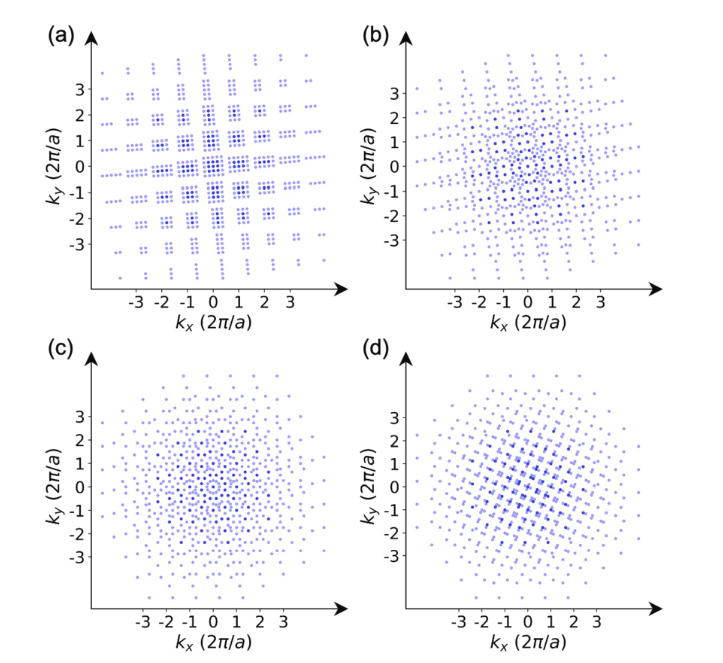
\includegraphics[width=0.95\textwidth]{./imgs/celdas.png}
        \end{center}
        \caption{\scriptsize{lattice reciproco para una red con huecos con angulos (a) $10^\circ$ (b) $20^\circ$ (c) $30^\circ$ (d) $40^\circ$. Imagen extraida de \cite{lou_fan_2025}}}
      \end{figure}
    \end{column}
    \end{columns}
  \end{frame}

\begin{frame}[allowframebreaks]
    \frametitle{RCWA4D nace como una modificación al método original para resolver casos rotados}
    \begin{itemize}
        \item \textbf{Expansión de la base:} En lugar de una red 2D, utiliza un conjunto de bases de ondas planas expandido que describe el carácter cuasi-periódico.
        \item \textbf{Red recíproca cuasi-4D ($G'$):} Los vectores de onda resultan de la combinación de los vectores de las redes recíprocas de cada capa individual ($g = g_1 + g_2$).
        \item \textbf{Eficiencia mediante dispersión (Sparsity):} Aunque el número de armónicos crece ($N^4$ en lugar de $N^2$), las matrices de convolución de cada capa son dispersas, lo que permite resolver el sistema sin formar matrices densas gigantes.
        \item \textbf{Ventaja:} Permite simular ángulos de giro arbitrarios e infinitesimales con una convergencia rápida.
    \end{itemize}
    
    \begin{center}
        % Si tienes acceso a la Fig 5 del paper original (diagrama de bloques diagonal)
        %\includegraphics[width=0.5\textwidth]{./imgs/sparsity_pattern.png}
      \textit{\small{RCWA4D transforma el problema de una supercelda inmensa en el espacio real a una red recíproca de mayor dimensión pero con operadores dispersos \cite{lou_fan_2025}.}}
    \end{center}
  \end{frame}


  % If you want to put references uncomment the lines below and the 
  \begin{frame}[t,allowframebreaks]
    \frametitle{References}
    \bibliographystyle{apalike}
    \bibliography{references}
  \end{frame}

\end{document}
